\documentclass[11pt,a4paper]{article}

\usepackage[T1]{fontenc}
\usepackage[utf8]{inputenc}
\usepackage{lmodern}
\usepackage{microtype}
\usepackage[margin=2.3cm]{geometry}
\usepackage{amsmath}
\usepackage{booktabs}
\usepackage{array}
\usepackage{tabularx}
\usepackage{longtable}
\usepackage{enumitem}
\usepackage{xcolor}
\usepackage{rotating}
\usepackage{float}
\usepackage{pgfplots}
\usepgfplotslibrary{groupplots}
\pgfplotsset{compat=1.18}
\usepackage{hyperref}

\definecolor{workinggreen}{HTML}{1B7F3A}
\definecolor{linkblue}{HTML}{1E5A96}

\hypersetup{
  colorlinks=true,
  linkcolor=linkblue,
  urlcolor=linkblue,
  citecolor=linkblue,
  pdftitle={LM-IDNet Adaptation Stage Report}
}

\setlength{\parindent}{0pt}
\setlength{\parskip}{0.65em}
\setlist[itemize]{topsep=0.25em,itemsep=0.2em,leftmargin=1.6em}
\setlist[enumerate]{topsep=0.25em,itemsep=0.2em,leftmargin=1.8em}
\renewcommand{\arraystretch}{1.2}

\newcommand{\projectname}{LM-IDNet}

\title{\textbf{LM-IDNet Adaptation Stage Report}\\
\large Architecture, Experiments, Findings, and Development Plan}
\author{Prepared for supervisor review}
\date{8 September 2026}

\begin{document}

\maketitle
\thispagestyle{empty}

\begin{abstract}
This report documents the complete adaptation stage currently implemented in
\projectname{}, a Dirichlet--multinomial anomaly detector for Internet of
Things traffic. It explains why adaptation was introduced, which data it uses,
how the static, threshold-only, and periodic-refitting systems differ, what
safeguards have been implemented, and how the experiments are reproduced. It
then reports the development results for Chromecast and Samsung smart-camera
traffic, including the initially disappointing adaptive results and the large
improvements obtained by changing the update cadence from 144 to 288 scored
windows and requiring 240 safe windows. The report deliberately separates a
promising development result from a final scientific claim. It also records
the observed contamination and parameter-stability problems that remain, and
sets out a focused plan for the next adaptation experiments.
\end{abstract}

\vfill
\begin{center}
\begin{minipage}{0.88\textwidth}
\small
\textbf{Scope and evidence.} This report covers only the adaptation stage. All
headline numbers are read from the stored model, event, adaptation, and
evaluation artefacts in the repository. The experiments use the declared
development-test partitions. Labels are used only after scoring for evaluation
and post-hoc diagnosis; they are never used to choose online updates. The
declared final-test captures remain outside this work.
\end{minipage}
\end{center}

\newpage
\tableofcontents
\newpage

\section{Executive Summary}

\subsection{Purpose of the adaptation stage}

A static anomaly detector assumes that the normal behaviour learned during
training remains appropriate indefinitely. Real IoT devices can change after
firmware updates, altered user routines, service changes, or network
reconfiguration. The purpose of adaptation is therefore to let the detector
respond to later benign behaviour without repeating the entire offline
training process.

Adaptation also creates a security risk. If attack traffic is accepted as
normal and used for updating, the detector can gradually learn the attack.
This is model poisoning. The adaptation stage was consequently developed as a
sequence of increasingly capable baselines rather than as an immediately
self-modifying production system:

\begin{enumerate}
  \item preserve the original static detector as the control;
  \item add threshold-only adaptation as a deliberately simple baseline;
  \item add guarded periodic refitting of the Dirichlet parameter vector
  $\boldsymbol{\alpha}$;
  \item vary the update timing and evidence requirement on development data;
  \item retain the strongest setting as a development candidate while
  documenting its remaining limitations.
\end{enumerate}

\subsection{Current outcome}

The adaptation infrastructure is operational. A configuration selects one of
three modes, all modes traverse the same chronological stream, all decisions
are recorded as ordinary anomaly events, and every adaptive update or rejection
is audited. The original static model and threshold artefacts are never
overwritten.

The first adaptive settings used a 288-window buffer, attempted updates every
144 scored windows, required 144 safe windows for refitting, and used a safety
margin of one calibration-score interquartile range (IQR). Those settings did
not improve on the static detector. Periodic refitting only partly recovered
the loss caused by threshold-only adaptation on Chromecast and made no
difference to Samsung decisions.

An exploratory development sweep identified update timing as the dominant
control. Changing the update interval from 144 to 288 windows and requiring
240 safe windows produced the following stored result:

\begin{table}[ht]
\centering
\small
\begin{tabular}{lrrrrrr}
\toprule
\textbf{Device} & \textbf{TP} & \textbf{FP} & \textbf{FN} &
\textbf{Precision} & \textbf{Recall} & \textbf{F1} \\
\midrule
Chromecast & 23 & 2 & 9 & 92.00\% & 71.88\% & 80.70\% \\
Samsung camera & 46 & 3 & 24 & 93.88\% & 65.71\% & 77.31\% \\
\bottomrule
\end{tabular}
\caption{Selected periodic-refit development result with
\texttt{update\_every=288} and \texttt{minimum\_refit\_windows=240}.}
\label{tab:selected-headline}
\end{table}

For Chromecast, this setting exceeds the static development result on all
reported classification measures. For Samsung, it is close to static: it
removes one false positive but misses two additional attacks. These outcomes
are promising, but the timing was selected after examining development
performance and must not be presented as locked final-test evidence.

In summary, the 288/240 setting is the strongest development candidate, but
safe-buffer contamination and the large Samsung alpha change must be addressed
before the adaptive policy is frozen.

\section{Adaptation Requirements and Data Boundaries}

\subsection{What adaptation is expected to do}

At time $t$, the active detector consists of a Dirichlet parameter vector
$\boldsymbol{\alpha}_t$, a lower-tail anomaly threshold $\tau_t$, and a score
IQR used to normalise severity. The adaptation stage receives each later
non-missing count window in chronological order. It must first make an anomaly
decision with the state that was active when the window arrived. Only after
that decision may the window influence a later state.

This order prevents a window from changing the model that judges itself. The
desired adaptive behaviour is therefore:

\begin{center}
\fbox{score current window $\longrightarrow$ record decision
$\longrightarrow$ update buffers $\longrightarrow$ optionally update future state}
\end{center}

The static detector remains the immutable control and starting point for every
run. Adaptive outputs are isolated and never overwrite its model or threshold.

\subsection{Data used by each part of the system}

\begin{table}[ht]
\centering
\small
\begin{tabularx}{\textwidth}{>{\raggedright\arraybackslash}p{0.22\textwidth}
>{\raggedright\arraybackslash}p{0.24\textwidth} X}
\toprule
\textbf{Component} & \textbf{Data} & \textbf{Purpose} \\
\midrule
Initial model & Benign fit captures & Estimate the starting
$\boldsymbol{\alpha}_0$. \\
Initial threshold & Separate benign calibration captures & Estimate the
lower-tail threshold $\tau_0$ and calibration score IQR. \\
Adaptation stream & Chronological development-test captures & Produce
decisions and, depending on mode, update the threshold and model. \\
Safe refit buffer & Development windows accepted by the immutable static
safety gate & Fit candidate alpha parameters without using labels. \\
Evaluation & Development labels joined after scoring & Measure TP, TN, FP,
FN, accuracy, precision, recall, and F1. \\
Final-test captures & Not used & Reserved until adaptation choices are frozen.
\\
\bottomrule
\end{tabularx}
\caption{Data ownership in the adaptation study.}
\label{tab:data-ownership}
\end{table}

Missing windows are skipped because they contain no observation. Observed
silent windows remain legitimate zero-count observations and are scored. All
experiments use the same device-specific development capture IDs, category
ordering, ten-minute aggregation, raw anomaly score, and initial model and
threshold artefacts.

\section{Implemented Adaptation Architecture}

\subsection{Configuration-selected systems}

The same scoring path supports three detector modes:

\begin{description}[style=nextline,leftmargin=3.8cm,labelwidth=3.5cm]
  \item[\texttt{static}] Keep alpha, threshold, score IQR, expected profile,
  and model fingerprint fixed for the complete stream.
  \item[\texttt{adaptive\_threshold}] Keep alpha fixed but periodically
  replace the threshold and score IQR using recent scores.
  \item[\texttt{periodic\_refit}] Perform the threshold adaptation baseline
  and additionally fit guarded candidate alpha vectors at the same update
  cadence.
\end{description}

This arrangement avoids separate programs whose preprocessing or scoring
details could drift apart. Experiments differ through JSON configuration and
isolated output paths. The shell runner executes the systems with the same
command sequence.

\subsection{Threshold-only adaptation baseline}

Threshold-only mode maintains a bounded deque of the latest non-missing
scores. After every configured number $M$ of scored windows, and after the
buffer has at least the configured calibration minimum, it calculates

\[
\tau_{t+1}=Q_q(S_t),
\qquad
\operatorname{IQR}_{t+1}=Q_{0.75}(S_t)-Q_{0.25}(S_t),
\]

where $S_t$ is the recent score buffer and $q=0.01$ in the reported
experiments. If the candidate IQR is not positive, the update is rejected and
the existing threshold remains active.

This mode is intentionally naive. It uses all recent scores, including scores
from windows currently classified as anomalous, and does not use labels. Its
purpose is to show whether moving the decision threshold alone is sufficient.
The later periodic mode retains this threshold policy so that the additional
effect of alpha refitting can be measured against it.

\subsection{High-confidence safety gate}

Periodic-refit mode maintains a second bounded deque containing candidate safe
count windows. A window enters this buffer only if its score under the
\emph{original static model and threshold} satisfies

\[
s_0(\mathbf{x}_t)
\geq
\tau_0 + m\,\operatorname{IQR}_0,
\]

where $m$ is \texttt{safe\_margin}. The experiments use $m=1$. The immutable
static score is deliberately used even after promotion. This prevents a
progressively relaxed adaptive model from admitting its own increasingly broad
set of training observations.

The gate is conservative against gradual self-approval, but it has a known
ceiling: an attack that already appears normal to the original model can still
enter the safe buffer. Section~\ref{sec:safety-findings} measures this problem.

\subsection{Periodic candidate fitting}

At each update interval, periodic mode performs the following procedure:

\begin{enumerate}
  \item Confirm that the recent-score buffer has at least the calibration
  minimum and the safe buffer has at least
  \texttt{minimum\_refit\_windows} observations.
  \item Add one one-hot smoothing row for each of TCP, UDP, SSDP, and ARP.
  These four minimal pseudo-observations prevent a temporarily absent protocol
  from forcing its alpha value to zero, which the Dirichlet model forbids.
  \item Reuse the existing fixed-point Dirichlet--multinomial estimator to fit
  a candidate $\boldsymbol{\alpha}^{*}$ on this guarded matrix.
  \item Compare the active and candidate likelihoods on the same guarded
  matrix.
  \item Rescore the recent raw count buffer under the candidate alpha and
  compute a matching candidate threshold and IQR.
  \item Promote all dependent state together, or reject the complete candidate.
\end{enumerate}

Promotion requires all of the following:

\begin{itemize}
  \item the estimator converged;
  \item the candidate likelihood is not worse than the active-model likelihood
  beyond numerical tolerance;
  \item the candidate recent-score IQR is positive.
\end{itemize}

If candidate fitting fails, does not converge, loses likelihood, or yields an
invalid score IQR, alpha remains unchanged. The detector then attempts the
ordinary threshold-only update under the active model. This makes failure
recoverable and keeps the baseline behaviour available.

\subsection{Atomic model identity and audit trail}

Alpha, concentration-derived expected proportions, model fingerprint,
threshold, and score IQR are promoted atomically. Scores already emitted are
not rewritten. Every later event carries the fingerprint of the model that
actually scored it.

The adaptation report stores:

\begin{itemize}
  \item initial and final alpha vectors and model fingerprints;
  \item initial and final thresholds and score IQR values;
  \item buffer sizes, update cadence, safety margin, and safe-window count;
  \item each threshold attempt, its position in the stream, old and new state,
  promotion status, and rejection reason;
  \item each model-refit attempt, convergence details, likelihood comparison,
  old and new alpha, and promotion status.
\end{itemize}

This record supports post-hoc inspection without overwriting the offline model.
It is an experimental audit trail rather than a production rollback store.

\section{Experiment Design}

\subsection{Devices and comparable streams}

The adaptation experiments use two labelled UNSW device datasets:

\begin{itemize}
  \item \textbf{Chromecast:} development captures 20--23 October 2018,
  producing 474 matched scored windows, including 32 labelled attack windows.
  \item \textbf{Samsung smart camera:} development captures 1--4 June 2018,
  producing 556 matched scored windows, including 70 labelled attack windows.
\end{itemize}

For every stored detector variant, the capture IDs, window timestamps, and
count vectors align exactly. Evaluation reports contain zero unmatched scores
and zero unmatched labels. This makes differences attributable to detector
state rather than different dataset composition.

\subsection{Stored experiment variants}

Four systems are stored for each device:

\begin{longtable}{>{\raggedright\arraybackslash}p{0.22\textwidth}
>{\raggedright\arraybackslash}p{0.20\textwidth}
>{\raggedright\arraybackslash}p{0.16\textwidth}
>{\raggedright\arraybackslash}p{0.16\textwidth}
>{\raggedright\arraybackslash}p{0.16\textwidth}}
\caption{Adaptation experiment variants.}\label{tab:variants}\\
\toprule
\textbf{Variant} & \textbf{Mode} & \textbf{Buffer} &
\textbf{Update interval} & \textbf{Minimum safe} \\
\midrule
\endfirsthead
\toprule
\textbf{Variant} & \textbf{Mode} & \textbf{Buffer} &
\textbf{Update interval} & \textbf{Minimum safe} \\
\midrule
\endhead
Static baseline & \texttt{static} & Not used & Not used & Not used \\
Adaptive-threshold baseline & \texttt{adaptive\_threshold} & 288 & 144 & Not used \\
Initial periodic refit & \texttt{periodic\_refit} & 288 & 144 & 144 \\
Selected periodic 288/240 & \texttt{periodic\_refit} & 288 & 288 & 240 \\
\bottomrule
\end{longtable}

All adaptive variants retain \texttt{safe\_margin=1.0}, calibration quantile
0.01, and raw scoring. The static result is generated from the versioned device
configuration. Adaptive variants use independent event and report directories,
so one run cannot erase another system's evidence.

\subsection{Execution interface}

The complete experiment runner is:

\begin{verbatim}
/bin/sh /home/usrtima/projects/iot_anomaly_detection/
  scripts/run_adaptation_experiments.sh
\end{verbatim}

The line break above is for presentation; the command is entered on one line.
The script resolves the repository root from its own location, so it also works
when launched from another current directory. It trains, calibrates, scores,
and evaluates the static systems, then runs and evaluates every matching
threshold and periodic-refit experiment configuration.

An individual selected experiment can be rerun with:

\begin{verbatim}
./scripts/run.sh adapt --config \
  configs/experiments/unsw_chromecast_periodic_refit_288_240.json
./scripts/run.sh evaluate --config \
  configs/experiments/unsw_chromecast_periodic_refit_288_240.json
\end{verbatim}

The Samsung commands use the corresponding Samsung configuration filename.

\section{Experimental Results}

\subsection{Complete development comparison}

\begin{sidewaystable}[p]
\centering
\small
\begin{tabular}{llrrrrrrrr}
\toprule
\textbf{Device} & \textbf{System} & \textbf{TP} & \textbf{TN} &
\textbf{FP} & \textbf{FN} & \textbf{Accuracy} & \textbf{Precision} &
\textbf{Recall} & \textbf{F1} \\
\midrule
Chromecast & Static & 15 & 440 & 2 & 17 & 95.99\% & 88.24\% & 46.88\% & 61.22\% \\
Chromecast & Threshold only, 144 & 13 & 440 & 2 & 19 & 95.57\% & 86.67\% & 40.63\% & 55.32\% \\
Chromecast & Periodic, 144/144 & 14 & 440 & 2 & 18 & 95.78\% & 87.50\% & 43.75\% & 58.33\% \\
Chromecast & Periodic, 288/240 & 23 & 440 & 2 & 9 & 97.68\% & 92.00\% & 71.88\% & 80.70\% \\
\midrule
Samsung & Static & 48 & 482 & 4 & 22 & 95.32\% & 92.31\% & 68.57\% & 78.69\% \\
Samsung & Threshold only, 144 & 27 & 483 & 3 & 43 & 91.73\% & 90.00\% & 38.57\% & 54.00\% \\
Samsung & Periodic, 144/144 & 27 & 483 & 3 & 43 & 91.73\% & 90.00\% & 38.57\% & 54.00\% \\
Samsung & Periodic, 288/240 & 46 & 483 & 3 & 24 & 95.14\% & 93.88\% & 65.71\% & 77.31\% \\
\bottomrule
\end{tabular}
\caption{Stored development results for all adaptation variants.}
\label{tab:all-results}
\end{sidewaystable}

Accuracy is included but is not the primary selection measure because benign
windows outnumber attack windows. Recall, F1, and the absolute false-positive
and false-negative counts provide a more useful account of the trade-off.

\textbf{Threshold-only baseline.} Threshold adaptation reduced performance on
both devices. It lost two Chromecast true positives without removing a false
positive, while Samsung lost 21 true positives to remove one false positive;
the harmful Samsung threshold movement began at window 144.

\textbf{Initial periodic-refit baseline.} With the 144-window cadence, two of
three candidates were promoted for each device. Refitting recovered one
Chromecast true positive over threshold-only adaptation, but Samsung decisions
were unchanged, so neither periodic result surpassed static.

\subsection{Exploratory cadence sensitivity}

Update cadence was then varied on the same development streams with a
288-window buffer, a 144-window minimum safe count, and safety margin 1.0. This
was exploratory tuning: intermediate outputs were temporary, while the selected
288/240 setting was subsequently rerun and stored as a named experiment.

\begin{figure}[H]
\centering
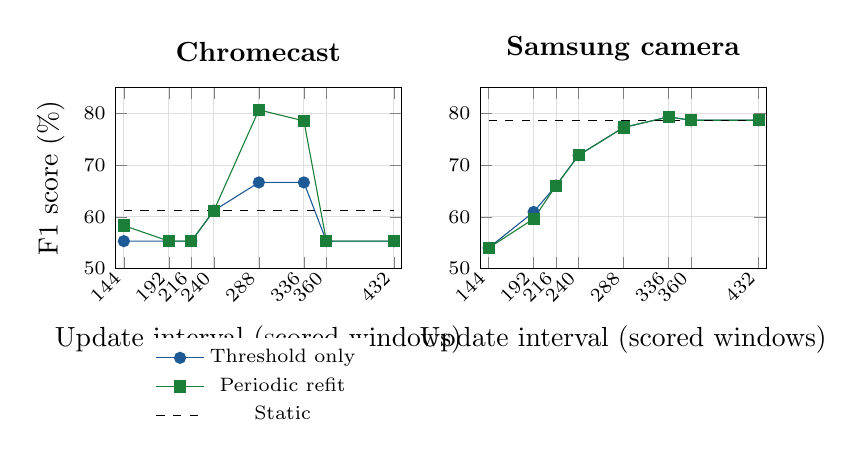
\begin{tikzpicture}
\begin{groupplot}[
  group style={group size=2 by 1, horizontal sep=1cm},
  width=0.43\textwidth,
  height=0.32\textwidth,
  xmin=135,
  xmax=440,
  ymin=50,
  ymax=85,
  xtick={144,192,216,240,288,336,360,432},
  x tick label style={font=\scriptsize,rotate=45,anchor=east},
  y tick label style={font=\scriptsize},
  grid=major,
  grid style={gray!25},
  xlabel={Update interval (scored windows)},
  ylabel={F1 score (\%)},
  title style={font=\bfseries},
  legend style={font=\scriptsize,draw=none,at={(0.5,-0.38)},anchor=north},
]
\nextgroupplot[title={Chromecast}]
\addplot[color=linkblue,mark=*] coordinates {
  (144,55.32) (192,55.32) (216,55.32) (240,61.22)
  (288,66.67) (336,66.67) (360,55.32) (432,55.32)
};
\addlegendentry{Threshold only}
\addplot[color=workinggreen,mark=square*] coordinates {
  (144,58.33) (192,55.32) (216,55.32) (240,61.22)
  (288,80.70) (336,78.57) (360,55.32) (432,55.32)
};
\addlegendentry{Periodic refit}
\addplot[color=black,dashed] coordinates {(144,61.22) (432,61.22)};
\addlegendentry{Static}

\nextgroupplot[title={Samsung camera},ylabel={}]
\addplot[color=linkblue,mark=*] coordinates {
  (144,54.00) (192,60.95) (216,66.06) (240,71.93)
  (288,77.31) (336,79.34) (360,78.69) (432,78.69)
};
\addplot[color=workinggreen,mark=square*] coordinates {
  (144,54.00) (192,59.62) (216,66.06) (240,71.93)
  (288,77.31) (336,79.34) (360,78.69) (432,78.69)
};
\addplot[color=black,dashed] coordinates {(144,78.69) (432,78.69)};
\end{groupplot}
\end{tikzpicture}
\caption{Exploratory F1 sensitivity to the update cadence.}
\label{fig:cadence-sweep}
\end{figure}

The cadence effect is much larger than the buffer-capacity or minimum-safe
effects. At the 144-window cadence, increasing the buffer from 288 to 432 raised
Chromecast periodic F1 from 58.33\% to 64.00\% but did not change Samsung.
Changing the minimum safe count from 144 to 240 did not change decisions in the
tested settings because enough safe windows were already available at the
promoted updates. Setting the minimum to 288 blocked useful Chromecast
refitting at the first opportunity because only 285 safe windows were present.

The value 288 was selected instead of 336 even though 336 had the highest
Samsung F1. Two hundred and eighty-eight ten-minute windows represent a clear
two-day nominal cadence, whereas 336 was an arbitrary development optimum more
likely to encode the particular attack schedule. This choice is an attempt to
retain a meaningful operational interpretation rather than maximising one
table entry.

\subsection{Improvement from the selected 288/240 setting}

Compared with the initial periodic 144/144 setting, the selected configuration
produced:

\begin{table}[ht]
\centering
\small
\begin{tabular}{lrrrr}
\toprule
\textbf{Device} & \textbf{Additional TP} & \textbf{Fewer FN} &
\textbf{Recall change} & \textbf{F1 change} \\
\midrule
Chromecast & $+9$ & $-9$ & $+28.13$ points & $+22.37$ points \\
Samsung camera & $+19$ & $-19$ & $+27.14$ points & $+23.31$ points \\
\bottomrule
\end{tabular}
\caption{Improvement of selected periodic configuration over initial periodic
configuration. False-positive counts were unchanged.}
\label{tab:tuning-improvement}
\end{table}

Compared with static, selected periodic refitting found eight additional
Chromecast attacks at the same false-positive count. On Samsung it found two
fewer attacks but removed one false positive. This means the selected setting
is clearly stronger on Chromecast and approximately competitive, rather than
clearly superior, on Samsung.

The selected runs each attempted and promoted one model refit at window 288.
Chromecast used 285 safe windows and Samsung used 241. The candidate likelihood
improved on the guarded fitting matrix in both cases. This is evidence that the
fitting algorithm optimised its immediate objective, not proof that the
candidate generalises or is free from contamination.

\section{Safety and Stability Findings}
\label{sec:safety-findings}

\subsection{Post-hoc safe-buffer contamination}

After the unsupervised runs were complete, development labels were joined to
the safe-window identities to measure how well the gate had worked. This audit
does not introduce label leakage into adaptation because the labels were not
available to the updating algorithm.

\begin{table}[ht]
\centering
\small
\begin{tabular}{llrrr}
\toprule
\textbf{Device} & \textbf{Update} & \textbf{Safe windows} &
\textbf{Attack windows} & \textbf{Contamination} \\
\midrule
Chromecast & Window 288 & 285 & 0 & 0.00\% \\
Chromecast & Window 432 & 288 & 3 & 1.04\% \\
Samsung camera & Window 288 & 241 & 22 & 9.13\% \\
Samsung camera & Window 432 & 288 & 20 & 6.94\% \\
\bottomrule
\end{tabular}
\caption{Label-based diagnostic of buffers accepted by the static safety gate
in the initial periodic experiment.}
\label{tab:contamination}
\end{table}

The Samsung attack windows admitted at the first promoted refit include
Ping-of-Death, Smurf, TCP SYN, and UDP attack labels. The issue is therefore not
limited to one isolated label type. These windows are high-scoring under the
four-category static composition model, which means a stronger margin cannot
necessarily separate them.

An explicit margin check supports that conclusion. At Samsung window 288,
margins from zero through five IQR all retained 241 safe windows including the
same 22 attacks. A margin of ten IQR retained 239 windows and still included 21
attacks. Raising \texttt{safe\_margin} is therefore not the priority remedy.

\subsection{Alpha concentration movement}

The expected category mixture depends on the ratios
$\alpha_k/\alpha_0$, while the concentration
$\alpha_0=\sum_k\alpha_k$ controls dispersion. A refit can therefore alter
score behaviour substantially even when mean proportions move only modestly.

\begin{table}[ht]
\centering
\small
\begin{tabular}{llrrr}
\toprule
\textbf{Device} & \textbf{Experiment} & \textbf{Initial $\alpha_0$} &
\textbf{Final $\alpha_0$} & \textbf{Ratio} \\
\midrule
Chromecast & Initial periodic & 28.10 & 36.05 & 1.28 \\
Chromecast & Selected 288/240 & 28.10 & 34.47 & 1.23 \\
Samsung camera & Initial periodic & 17.39 & 206.40 & 11.87 \\
Samsung camera & Selected 288/240 & 17.39 & 166.62 & 9.58 \\
\bottomrule
\end{tabular}
\caption{Concentration movement under periodic refitting.}
\label{tab:concentration}
\end{table}

The Samsung movement remains very large even in the selected experiment. Its
mean traffic mixture changes much less dramatically than its concentration,
but the score distribution changes enough for the matching threshold to move
from $-16.9221$ to $-382.9139$. That absolute threshold should not be compared
directly with the static threshold because the underlying alpha and score scale
have changed. Decisions and classification metrics are the valid comparison.

The magnitude nevertheless shows that candidate likelihood and convergence
are insufficient stability guards. A future update should limit how quickly
concentration can change or blend candidate and active alpha values.

\subsection{What the selected cadence really achieved}

The selected cadence leaves the static detector active for the first 288
scored windows. This directly avoids the harmful Samsung threshold change at
window 144. It then gives Chromecast one useful refit before its later attack
windows. The improvement is therefore understandable rather than mysterious.

It also creates a risk of optimistic timing selection. Most Samsung attack
windows occur before the first selected update. A different deployment stream
could place attacks immediately after an update and produce a different result.
For that reason, the report treats 288 as a meaningful development candidate,
not as a universally optimal period.

\section{Work Completed During the Adaptation Stage}

The work progressed through the following concrete milestones:

\begin{enumerate}
  \item \textbf{Defined the role of adaptation.} The stage was separated from
  offline fitting and calibration. Development traffic became the chronological
  adaptation stream, and the final partition remained unused.
  \item \textbf{Preserved the fixed detector.} Static scoring remains available
  through its original command and through adaptation mode selection.
  \item \textbf{Added configuration-driven architecture.} The three detector
  systems are selected with \texttt{adaptation.mode}, while buffer capacity,
  cadence, minimum safe evidence, and safety margin are explicit JSON values.
  \item \textbf{Implemented threshold-only adaptation.} The detector updates a
  bounded recent-score quantile after scoring the current window and rejects
  invalid IQR candidates.
  \item \textbf{Added reproducible experiment execution.} Separate device and
  variant configurations isolate outputs. The shell runner resolves the
  repository root, fixing the earlier failure when it was launched from the
  scripts directory.
  \item \textbf{Implemented periodic alpha refitting.} Safe and recent buffers,
  candidate fitting, convergence and likelihood checks, candidate rescoring,
  atomic promotion, fingerprints, and rejection auditing were added.
  \item \textbf{Handled sparse protocol buffers.} Four one-hot smoothing rows
  allow fitting when a real safe buffer temporarily contains no observation of
  one protocol.
  \item \textbf{Ran the initial comparison.} Static, threshold-only, and
  144/144 periodic systems were evaluated for Chromecast and Samsung.
  \item \textbf{Diagnosed the negative result.} Window-level comparison showed
  that Samsung's first threshold change caused most of the loss. Safe-buffer
  auditing found attack contamination, and parameter inspection found a large
  concentration jump.
  \item \textbf{Explored parameter sensitivity.} Cadence, buffer size, minimum
  safe count, and safety margin were examined on development data.
  \item \textbf{Stored the selected experiment.} New 288/240 configurations,
  events, adaptation reports, and evaluation reports were produced for both
  devices without replacing earlier evidence.
\end{enumerate}

The adaptation logic is covered by automated checks for static equivalence,
score-before-update ordering, successful model promotion, matching threshold
and model fingerprints, smoothing rows, and rejection of non-converged
candidates. Real-data runs additionally confirmed that both selected
experiments completed, promoted one candidate, and matched every scored window
to a label.

\section{Current Limitations}

The following limitations are important to state explicitly:

\begin{enumerate}
  \item \textbf{Recent-score threshold contamination.} Both adaptive systems
  calculate threshold candidates from all recent scores. An attack-heavy
  interval can therefore make later attacks easier to accept.
  \item \textbf{Incomplete poisoning protection.} The safe gate excludes
  obvious low-scoring anomalies, but attacks invisible to the original
  composition model can enter the refit buffer.
  \item \textbf{In-sample promotion likelihood.} Candidate and active
  likelihoods are compared on the same matrix used for fitting. This detects a
  failed optimiser but does not prove generalisation.
  \item \textbf{No alpha rate limit.} A converged candidate can make a very
  large concentration jump, as observed for Samsung.
  \item \textbf{No independent traffic-volume guard.} A four-category
  composition model may consider high-volume attacks normal when their
  proportions resemble benign traffic.
  \item \textbf{Runtime-only adaptive state.} New alpha values are audited but
  not saved as independently deployable model artefacts with a formal rollback
  pointer.
  \item \textbf{One development sequence per device.} The selected cadence may
  benefit from the location of attacks in these particular streams.
  \item \textbf{No locked final result.} All reported comparisons support model
  development only.
  \item \textbf{No uncertainty interval.} Small differences such as one
  recovered attack should not be over-interpreted without repeated temporal
  evidence.
\end{enumerate}

These limitations do not invalidate the stage. They define what the current
baseline demonstrates and what the next version must improve.

\section{Parameters and Ideas for Further Work}

\subsection{Existing configurable parameters}

\begin{table}[ht]
\centering
\small
\begin{tabularx}{\textwidth}{>{\raggedright\arraybackslash}p{0.23\textwidth}
>{\raggedright\arraybackslash}p{0.20\textwidth} X}
\toprule
\textbf{Parameter} & \textbf{Current candidate} & \textbf{Interpretation} \\
\midrule
\texttt{buffer\_size} & 288 & Maximum recent score, count, and safe-window
capacity. Larger buffers are steadier but slower to reflect genuine drift. \\
\texttt{update\_every} & 288 & Number of scored windows between update
attempts. This was the most influential tested parameter. \\
\texttt{minimum\_refit\_windows} & 240 & Minimum safe evidence before fitting.
It is deliberately below 288 because the gate accepted 285 Chromecast and 241
Samsung windows at the useful update. \\
\texttt{safe\_margin} & 1.0 IQR & Distance above the original threshold needed
for refitting. Larger tested margins did not solve Samsung contamination. \\
Calibration quantile & 0.01 & Lower-tail operating point. Increasing it may
raise recall at the cost of false positives, but requires complete recalibration
and a new static control for every value. \\
Score type & Raw & Raw scoring retains count-volume information. Normalised
scoring is available but should be treated as a separate modelling experiment.
\\
Window duration & 10 minutes & Shorter windows may expose short attacks but
require complete preprocessing, training, calibration, and comparison. \\
\bottomrule
\end{tabularx}
\caption{Existing parameters relevant to adaptation performance.}
\label{tab:parameters}
\end{table}

Estimator tolerance, iteration limit, numerical precision, backend, and random
seeds should not be tuned to improve detection metrics. They control numerical
correctness, convergence, or reproducibility rather than the intended decision
boundary.

\subsection{Proposed adaptation controls}

The following ideas are not yet implemented. They are ordered by their direct
connection to the observed failures:

\begin{enumerate}
  \item \textbf{Safe-only threshold candidates.} Recalculate the threshold from
  scores belonging to the guarded buffer rather than all recent windows. This
  directly targets the harmful threshold contamination demonstrated by
  Samsung. A fixed-threshold periodic-refit variant should also be included so
  the alpha effect can be isolated.
  \item \textbf{Alpha blending rate.} Introduce a small $\rho$ and promote
  \[
  \boldsymbol{\alpha}_{t+1}
  =(1-\rho)\boldsymbol{\alpha}_t+\rho\boldsymbol{\alpha}^{*},
  \]
  initially testing values such as 0.05, 0.10, and 0.25. The threshold must be
  recalculated under the blended model.
  \item \textbf{Maximum concentration ratio.} Reject or cap a candidate when
  $\alpha_0^{*}/\alpha_{0,t}$ exceeds a configured bound, initially 1.5 or 2.0.
  This would allow the moderate Chromecast change while stopping the observed
  Samsung jump.
  \item \textbf{Independent volume/rate guard.} Use a simple total-packet-count
  or rate detector alongside composition likelihood. A window should enter the
  safe buffer only when both detectors consider it ordinary. This addresses
  attacks whose category proportions look normal but whose traffic volume does
  not.
  \item \textbf{Quarantined promotion subset.} Split accepted windows into a
  fitting subset and a later comparison subset. Promote only if the candidate
  improves likelihood or calibration behaviour on data it did not fit.
  \item \textbf{Explicit persisted model versions and rollback.} If the work
  moves from offline experiments to continuous deployment, store each promoted
  model as an immutable artefact and maintain an active-version pointer.
\end{enumerate}

The first three ideas remain small extensions of the present system. A complex
drift-detection framework is not justified until these direct safeguards have
been tested.

\section{Planned Experimental Sequence}

The next work should preserve the current evidence and change one mechanism at
a time:

\begin{enumerate}
  \item Retain static, initial threshold-only, initial periodic, and selected
  288/240 outputs as frozen development comparisons.
  \item Add two threshold-source variants at the 288/240 cadence: safe-only
  thresholding and fixed threshold with periodic alpha refitting.
  \item Compare those variants using TP, FP, FN, precision, recall, F1, and
  decision changes by update phase. Continue reporting absolute counts.
  \item Add alpha blending and a concentration-ratio limit only after the
  threshold source has been isolated. Record candidate and promoted alpha so
  the guard can be audited.
  \item Add the simplest total-volume guard and repeat the post-hoc safe-buffer
  contamination audit. The target is fewer labelled attacks entering the
  buffer without starving it of benign windows.
  \item Select one configuration based on both devices, not the best result for
  either device in isolation.
  \item Freeze code, configuration, model fingerprints, and decision criteria.
  Only then use the declared final-test captures once.
\end{enumerate}

A credible successor should satisfy the following development criteria before
final testing:

\begin{itemize}
  \item improve or approximately preserve static F1 on both devices;
  \item improve recall without a disproportionate false-positive increase;
  \item show that gains occur after updates rather than only because updates
  were delayed beyond attacks;
  \item materially reduce safe-buffer attack contamination;
  \item bound alpha concentration changes;
  \item record every rejection and promotion reproducibly.
\end{itemize}

\section{Conclusions for Supervisor Presentation}

The adaptation stage now provides a reproducible progression from a fixed
detector to threshold adaptation and guarded periodic alpha refitting. It is
not merely an interface: models were actually refitted, fingerprints changed,
matching thresholds were recalculated, failed candidates were rejected safely,
and decisions were evaluated on aligned labelled windows.

The first result was negative and informative. A one-day update cadence caused
the Samsung threshold to absorb attack-heavy behaviour, reducing recall
sharply. Periodic refitting could not repair that decision boundary. Inspection
then showed two deeper issues: attacks could pass the static safety gate, and
Samsung candidate concentration could change by more than an order of
magnitude.

Parameter analysis showed that update cadence dominated the currently exposed
controls. A two-day, 288-window cadence with a 240-safe-window requirement
raised Chromecast F1 from 58.33\% to 80.70\% and Samsung F1 from 54.00\% to
77.31\% relative to the initial periodic configuration, with no increase in
false positives. This is the strongest stored adaptation result so far.

The correct claim is therefore measured: \projectname{} has an operational and
auditable adaptation baseline, and conservative timing substantially improves
its development performance. It does not yet have complete poisoning
resistance or a final validated adaptive policy. The next work is focused on
safe-only thresholding, bounded alpha movement, and an independent volume
guard before configuration freeze and final evaluation.

\appendix

\section{Repository Evidence Map}

\subsection{Configurations}

\begin{itemize}
  \item \path{configs/unsw_chromecast.json}
  \item \path{configs/unsw_samsung_camera.json}
  \item \path{configs/experiments/unsw_chromecast_adaptive_threshold.json}
  \item \path{configs/experiments/unsw_samsung_camera_adaptive_threshold.json}
  \item \path{configs/experiments/unsw_chromecast_periodic_refit.json}
  \item \path{configs/experiments/unsw_samsung_camera_periodic_refit.json}
  \item \path{configs/experiments/unsw_chromecast_periodic_refit_288_240.json}
  \item \path{configs/experiments/unsw_samsung_camera_periodic_refit_288_240.json}
\end{itemize}

\subsection{Selected adaptation and evaluation reports}

\begin{itemize}
  \item \path{reports/experiments/UNSW-Chromecast/periodic_refit_288_240/adaptation.json}
  \item \path{reports/experiments/UNSW-Chromecast/periodic_refit_288_240/evaluation_statistics.json}
  \item \path{reports/experiments/UNSW-Samsung-Camera/periodic_refit_288_240/adaptation.json}
  \item \path{reports/experiments/UNSW-Samsung-Camera/periodic_refit_288_240/evaluation_statistics.json}
\end{itemize}

Earlier threshold-only and initial periodic reports remain in the corresponding
\path{reports/experiments/UNSW-Chromecast/} and
\path{reports/experiments/UNSW-Samsung-Camera/} subdirectories. Event arrays
are stored under matching \path{artifacts/experiments/} paths.

\subsection{Implementation and operation}

\begin{itemize}
  \item \path{src/lm_idnet/config.py}: adaptation modes and parameter validation;
  \item \path{src/lm_idnet/models/scoring_stage.py}: static scoring, threshold
  updates, guarded refitting, promotion, and reporting;
  \item \path{src/lm_idnet/artifacts.py}: fingerprints for active parameter
  versions;
  \item \path{scripts/run_adaptation_experiments.sh}: reproducible multi-device
  experiment runner;
  \item \path{docs/configuration.md}: configuration semantics;
  \item \path{docs/command-line-interface.md}: command behaviour.
\end{itemize}

\section{Selected Configuration}

The adaptation section selected for the stored development candidate is:

\begin{verbatim}
"adaptation": {
  "mode": "periodic_refit",
  "buffer_size": 288,
  "update_every": 288,
  "minimum_refit_windows": 240,
  "safe_margin": 1.0
}
\end{verbatim}

With ten-minute windows, 288 scored windows correspond nominally to 48 hours.
Because missing windows are skipped, the elapsed wall-clock duration can be
longer. The cadence is therefore precisely a count of usable observations, not
a guaranteed clock schedule.

\end{document}
